\chapter{Défis techniques posés par le texte}\label{Défis}
%\chapterprecis{Où l'on se pose des questions.}
\section{Caractéristiques techniques du livre originel}\label{DéfisTech}
Le livre fait plus de 600 pages.
Il est imprimé sur du papier et relié de cuir.
%\section{Lecture des images sources}\label{DéfisLect}

\section{Caractères spéciaux}\label{DéfisCar}
Wilkins présente beaucoup de langues dans le cadre de sa démonstration.
Certaines de ces langues, comme l'allemand et le danois, ont d'autres caractéristiques typographiques que le texte alentours, par exemple elles sont composées en lettres gothiques.
Dans ses descriptions phonétiques, Wilkins utilise aussi des caractères spéciaux, comme la lettre 〈ɑ〉 (alpha latin, différent de 〈α〉 alpha grec), le digramme 〈ȣ〉 (pour 〈ou〉) et un 〈y〉 agrémenté d'une ligne souscrite.
Cette dernière lettre, qui contrairement aux autres n'est pas dans les spécifications Unicode, est remplacée dans la digitalisation EEB par 〈ƴ〉.
\subsection{Caractères non-latins}
\begin{figure}[h]
   \caption{\label{Chinese} Exemple de caractères chinois}
   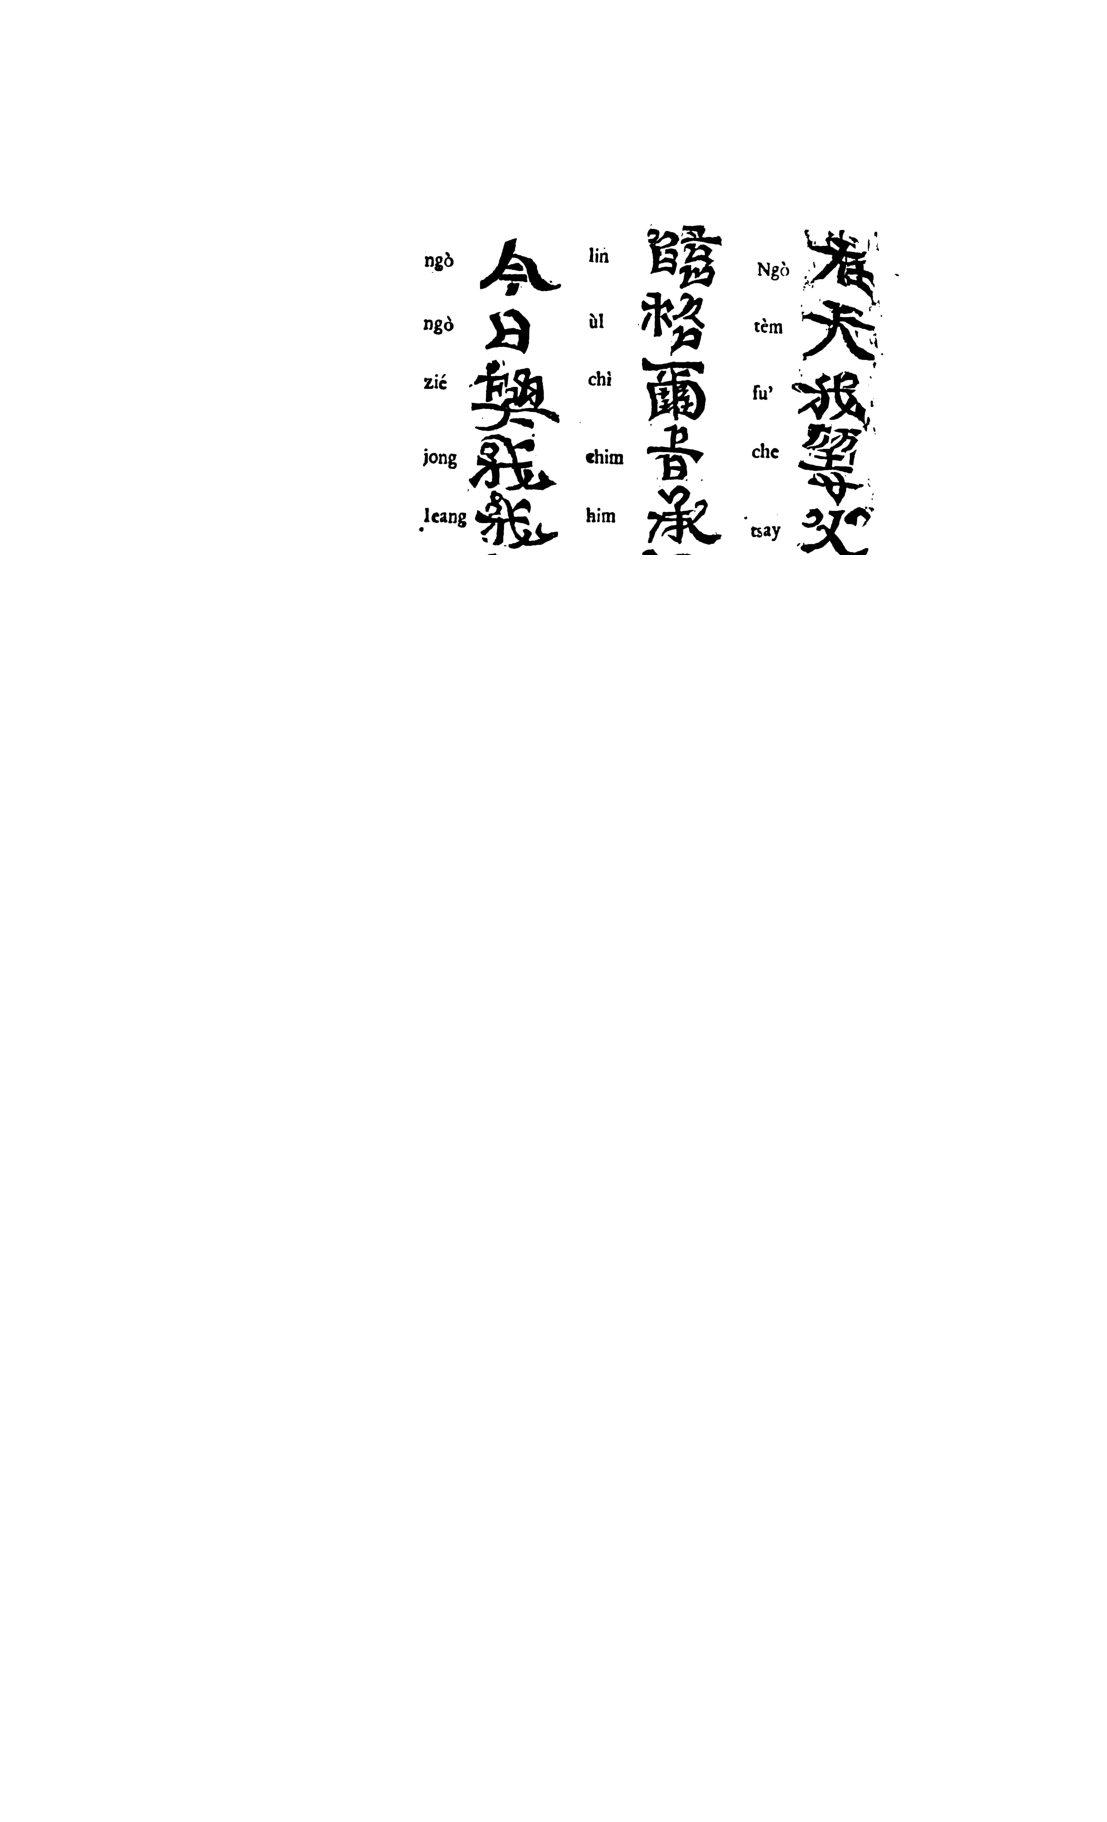
\includegraphics[scale=1]{Chinese}
\end{figure}
Un des tableaux donne des exemples de caractères chinois avec prononciation \parencite[p. 451]{wilkins_essay_1668}.
L'encodage d'Early English Books Online, pour chacun d'entre eux, signale \code{〈in non-Latin alphabet 〉}.
On perd ainsi de l'information, alors que de nos jours Unicode permet -- entre autres -- l'encodage de tous les systèmes d'écriture dérivés des logogrammes chinois.

Le problème est qu'à l'époque aucun imprimeur en Europe ne disposait de polices de caractères chinois, et ce qu'on retrouve dans ETRC sont des gravures faites à main levée.
Pour retrouver le caractère représenté, les recherches graphiques doivent être accompagnées de recherches phonétiques, en espérant que la romanisation fournie par Wilkins permette de retrouver quelle langue chinoise est ainsi décrite.

\subsection{L'écriture philosophique}
\begin{figure}[h]
   \caption{\label{LordsPrayer} Le Notre-Père}
   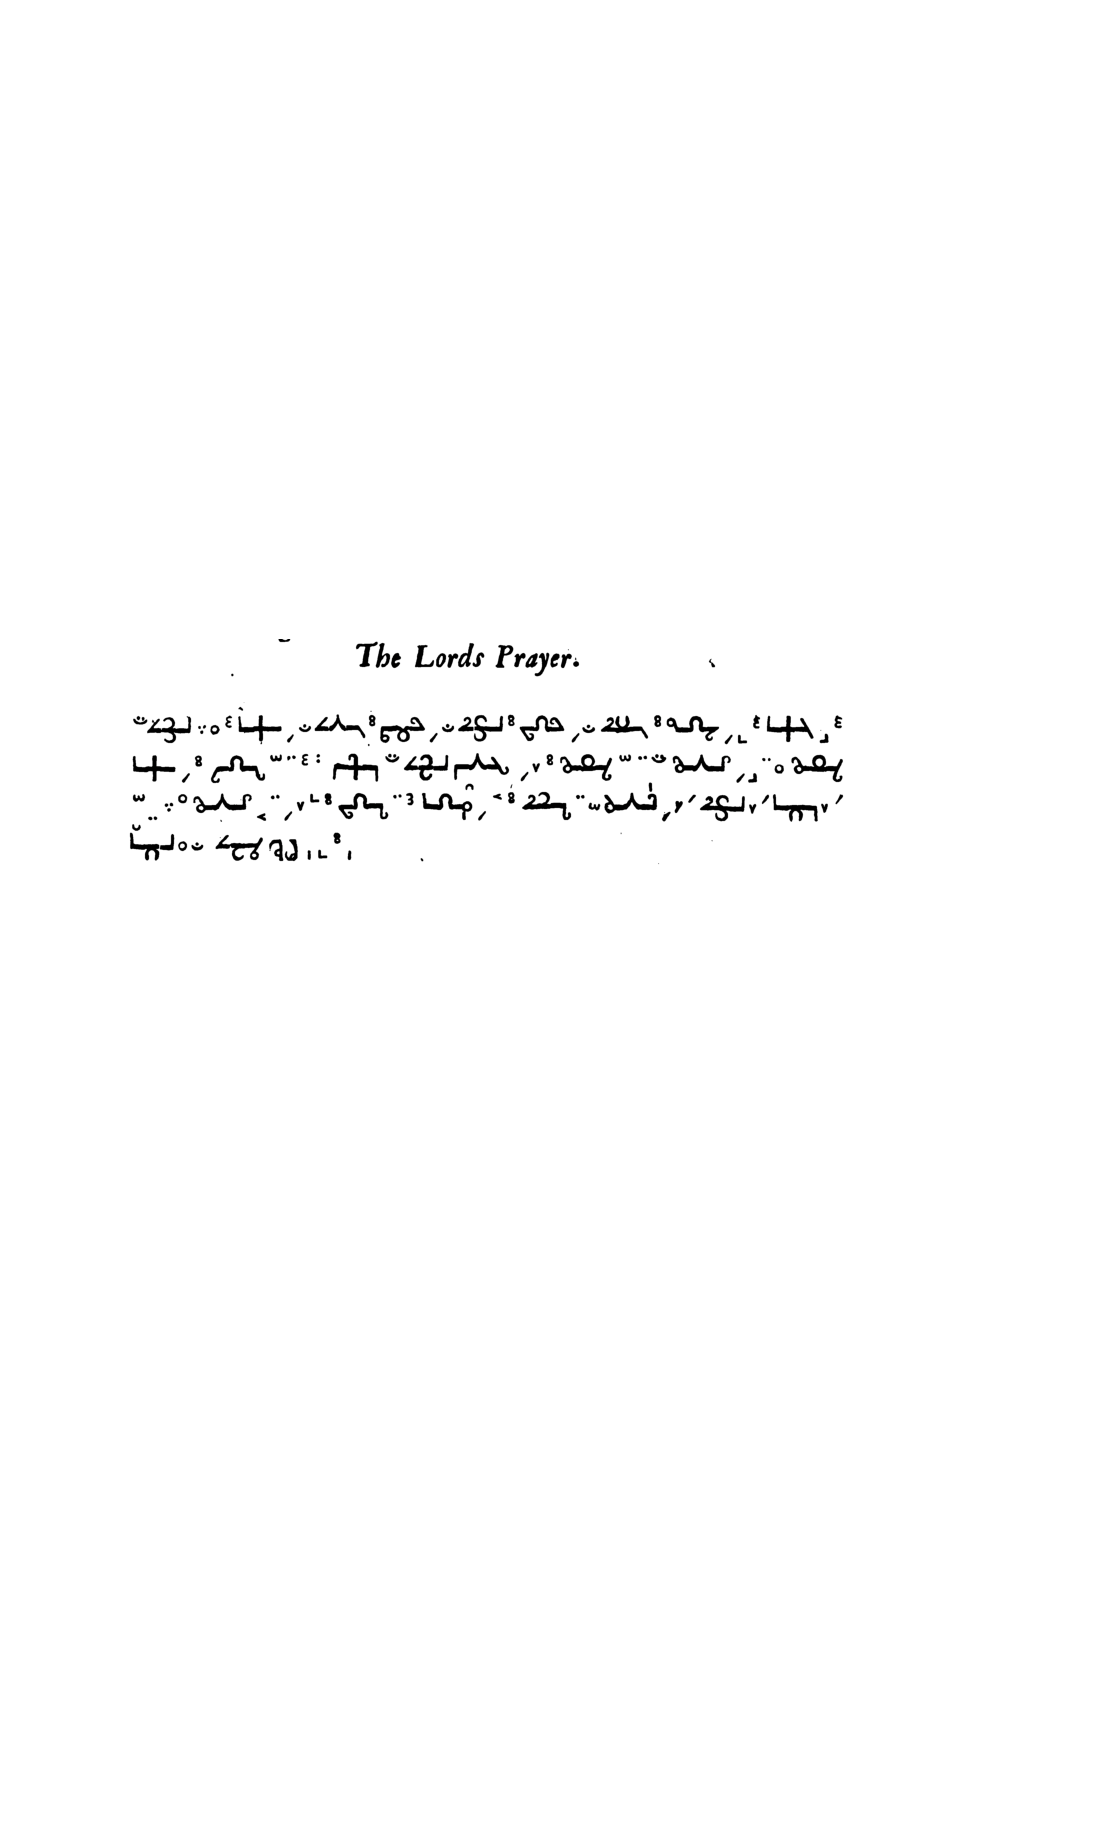
\includegraphics[scale=0.8]{LordsPrayer}
\end{figure}
En plus d'employer des systèmes d'écriture non-européens, Wilkins en invente un dans le cadre de sa recherche d'une langue parfaite, qu'il nomme \emph{real character}.
Il s'agit d'un système de nature idéographique : ses \og philosophical letters\fg{} sont composées de trois parties indiquant le \emph{genre}, la \emph{différence} et l'\emph{espèce} en accord avec le système de classification développé dans les chapitres précédents.
Des diacritiques viennent préciser la classe grammaticale, les inflexions verbales, le nombre.
De plus, des caractères spéciaux sont prévus pour les mots grammaticaux tels que la copule, les pronoms, les prépositions, les interjections \parencite[part. IV, chap. I]{wilkins_essay_1668}.

Ce système n'a pas encore été proposé à l'encodage chez Unicode.
De ce fait, il n'est pas possible de l'employer comme n'importe quel autre écriture dans un document électronique.
Une solution serait de trouver une police faisant correspondre les lettres d'un système existant aux caractères philosophiques.
Si pour l'impression d'ETRC en 1668 une police mécanique semble bien avoir été créée par le typographe Joseph Moxon \parencite{bryden_moxon_2004}, il n'en existe pas d'équivalent numérique à ce jour.
Il faudra donc partir de zéro.

La création typographique est en principe accessible à tous : à côté des logiciels d'édition commerciale comme FontLab\footnote{\url{http://www.fontlab.com}} utilisés par les professionnels, il existe des libres comme FontForge\footnote{\url{https://fontforge.github.io/en-US/}} avec les mêmes fonctionnalités.
Cependant, le design d'une police demande une certaine expérience, non seulement pour obtenir un aspect visuellement harmonieux, mais aussi, dans le cas de l'écriture philosophique de Wilkins, pour construire les ligatures qui rassemblent les éléments basiques en caractères uniques.

\section{Images}\label{DéfisImages}
L'ouvrage de base est illustré (présence de gravures) et décoré (en-têtes de chapitres, lettrines).
On désire que ces images, ou des approximations remplissant la même fonction, soient présentes dans l'édition finale.

La page 378, par exemple, présente un tableau consistant en trente-cinq vignettes représentant un visage d'homme de face et en coupe latérale articulant les consonnes et les voyelles décrites dans la partie III.
Les distinctions sont très fines, malheureusement les PDF de la numérisation par Google Books utilisent un contraste noir-blanc trop violent qui efface les détails ; et même l'image en ligne n'a pas de grain assez fin pour être satisfaisant.
L'exemple ci-devant est tiré de la numérisation depuis l'exemplaire de la bibliothèque de l'État de Bavière.
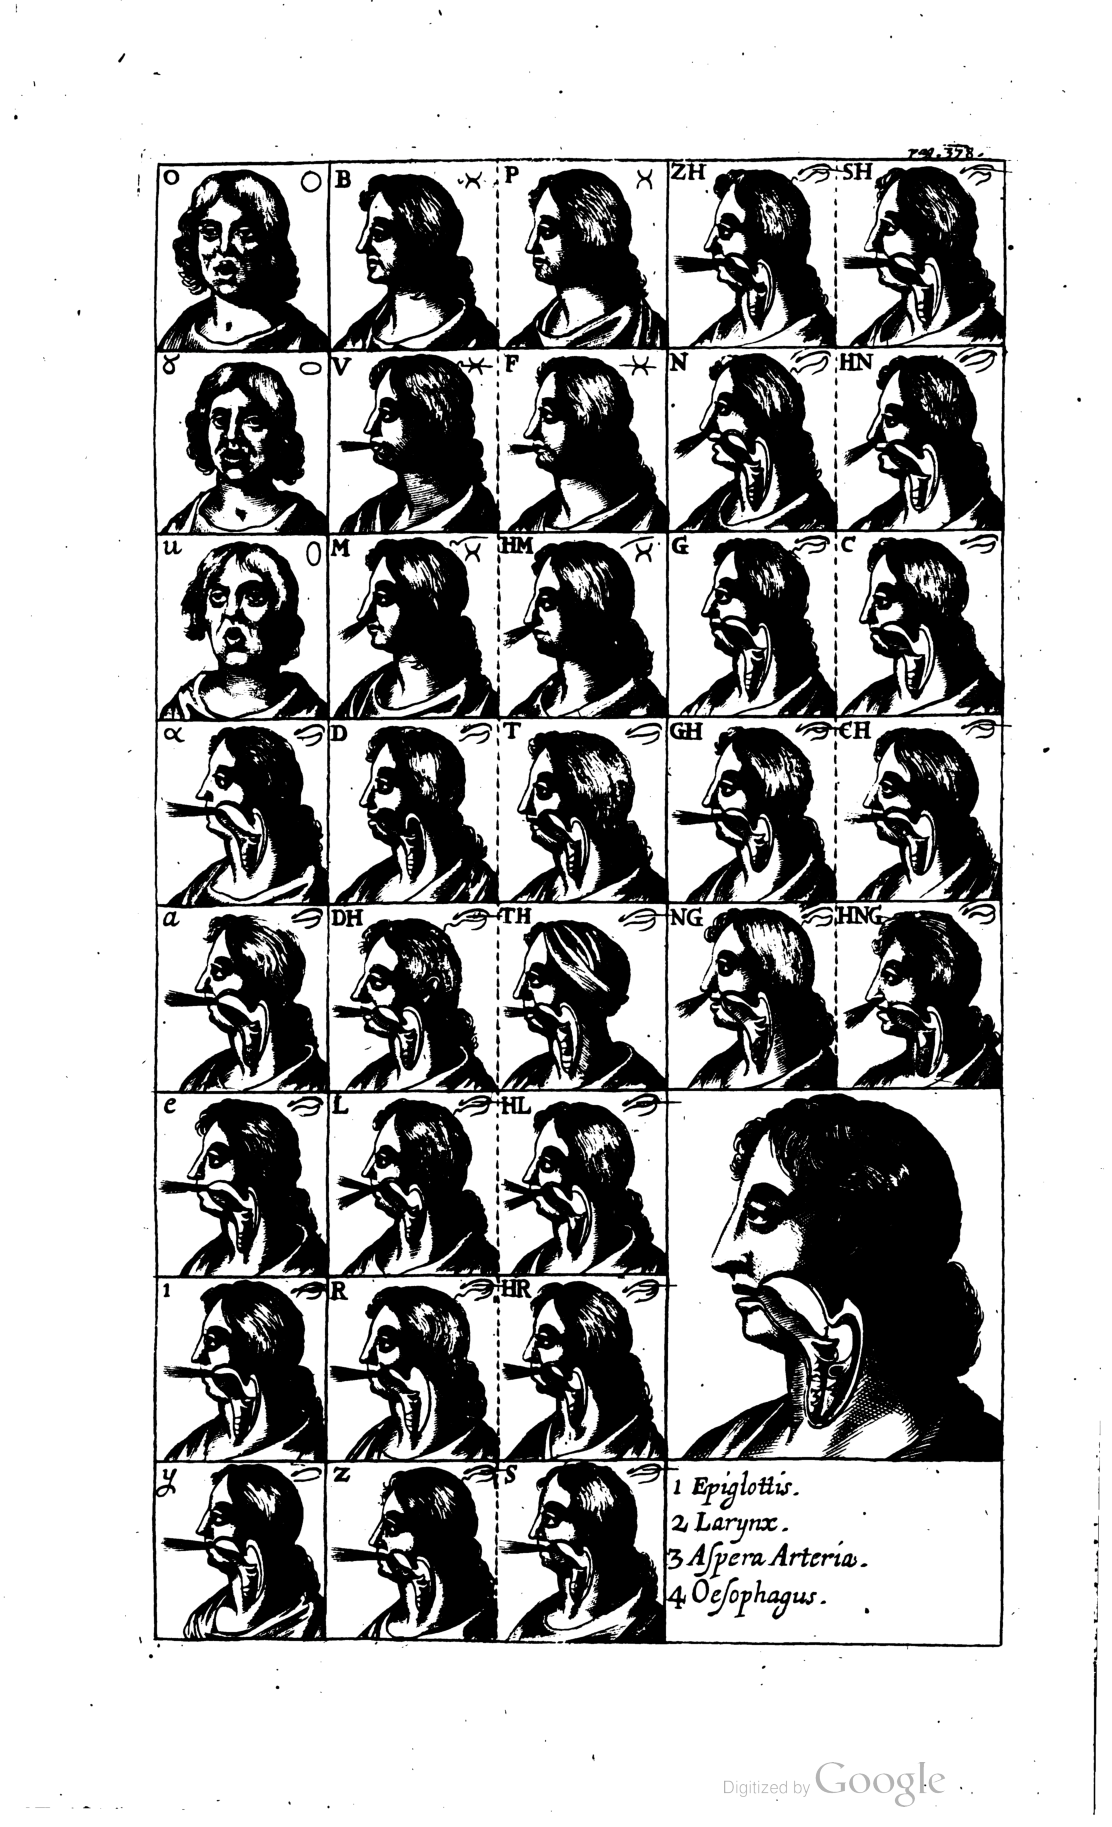
\includepdf{Articulations}
Dans ces conditions, comment obtenir des images de meilleure qualité ?
On pourrait réaliser une nouvelle reproduction à partir de l'original avec des appareils de meilleur qualité.
Mais peut-être que recréer ces images, les moderniser tout en en conservant les principes de construction, rendrait la version électronique plus harmonieuse.
\section{Liens}\label{DéfisLiens}
Des renvois sont faits dans le texte vers l'intérieur et l'extérieur de celui-ci.
Il est possible d'en faire des liens dynamiques.
	\subsection{Liens internes}
Tant que chaque division du livre est correctement signalée à l'aide de balises imbriquées, il est possible de leur attribuer un identifiant unique avec l'attribut \code{@xml:id} auquel on peut renvoyer par un attribut \code{@target} se trouvant dans une balise \code{<ref>}, laquelle encadre la référence à la division dans le texte.
	\subsection{Liens externes}
Wilkins cite beaucoup d'ouvrages et chapitres d'ouvrages qu'il a pu consulter pour la rédaction de son essai, sur des sujets linguistiques et philosophiques.
Lorsque des versions électroniques existent en ligne, par exemple sur une des plate-formes mentionnée en section \ref{}\ref{HistDigitEmp}, on aimerait pouvoir y renvoyer le lecteur.